\chapter{Experiment}
Sensor:\\
Hokuyo UBG 04-LX - 2D scanning laser rangefinder. Measures range\\

Robot arm: \\
Kinova Jaco - can program to move with and record pose

Target object: \\
$0.1 \times 0.1$ m MDF cube, spray painted matte white

1. Collected measurements to model sensor noise for simulation\\
2. Collected measurements of moving cube + measured ground truth cube state - for testing observer with real world conditions

\section{Sensor Noise Characterisation}
	\subsection{Setup}
		physical setup\\
		measurement configurations 
	\subsection{Results}
		data\\
		Histograms - range error approximately normally distributed:
		\begin{figure}
		  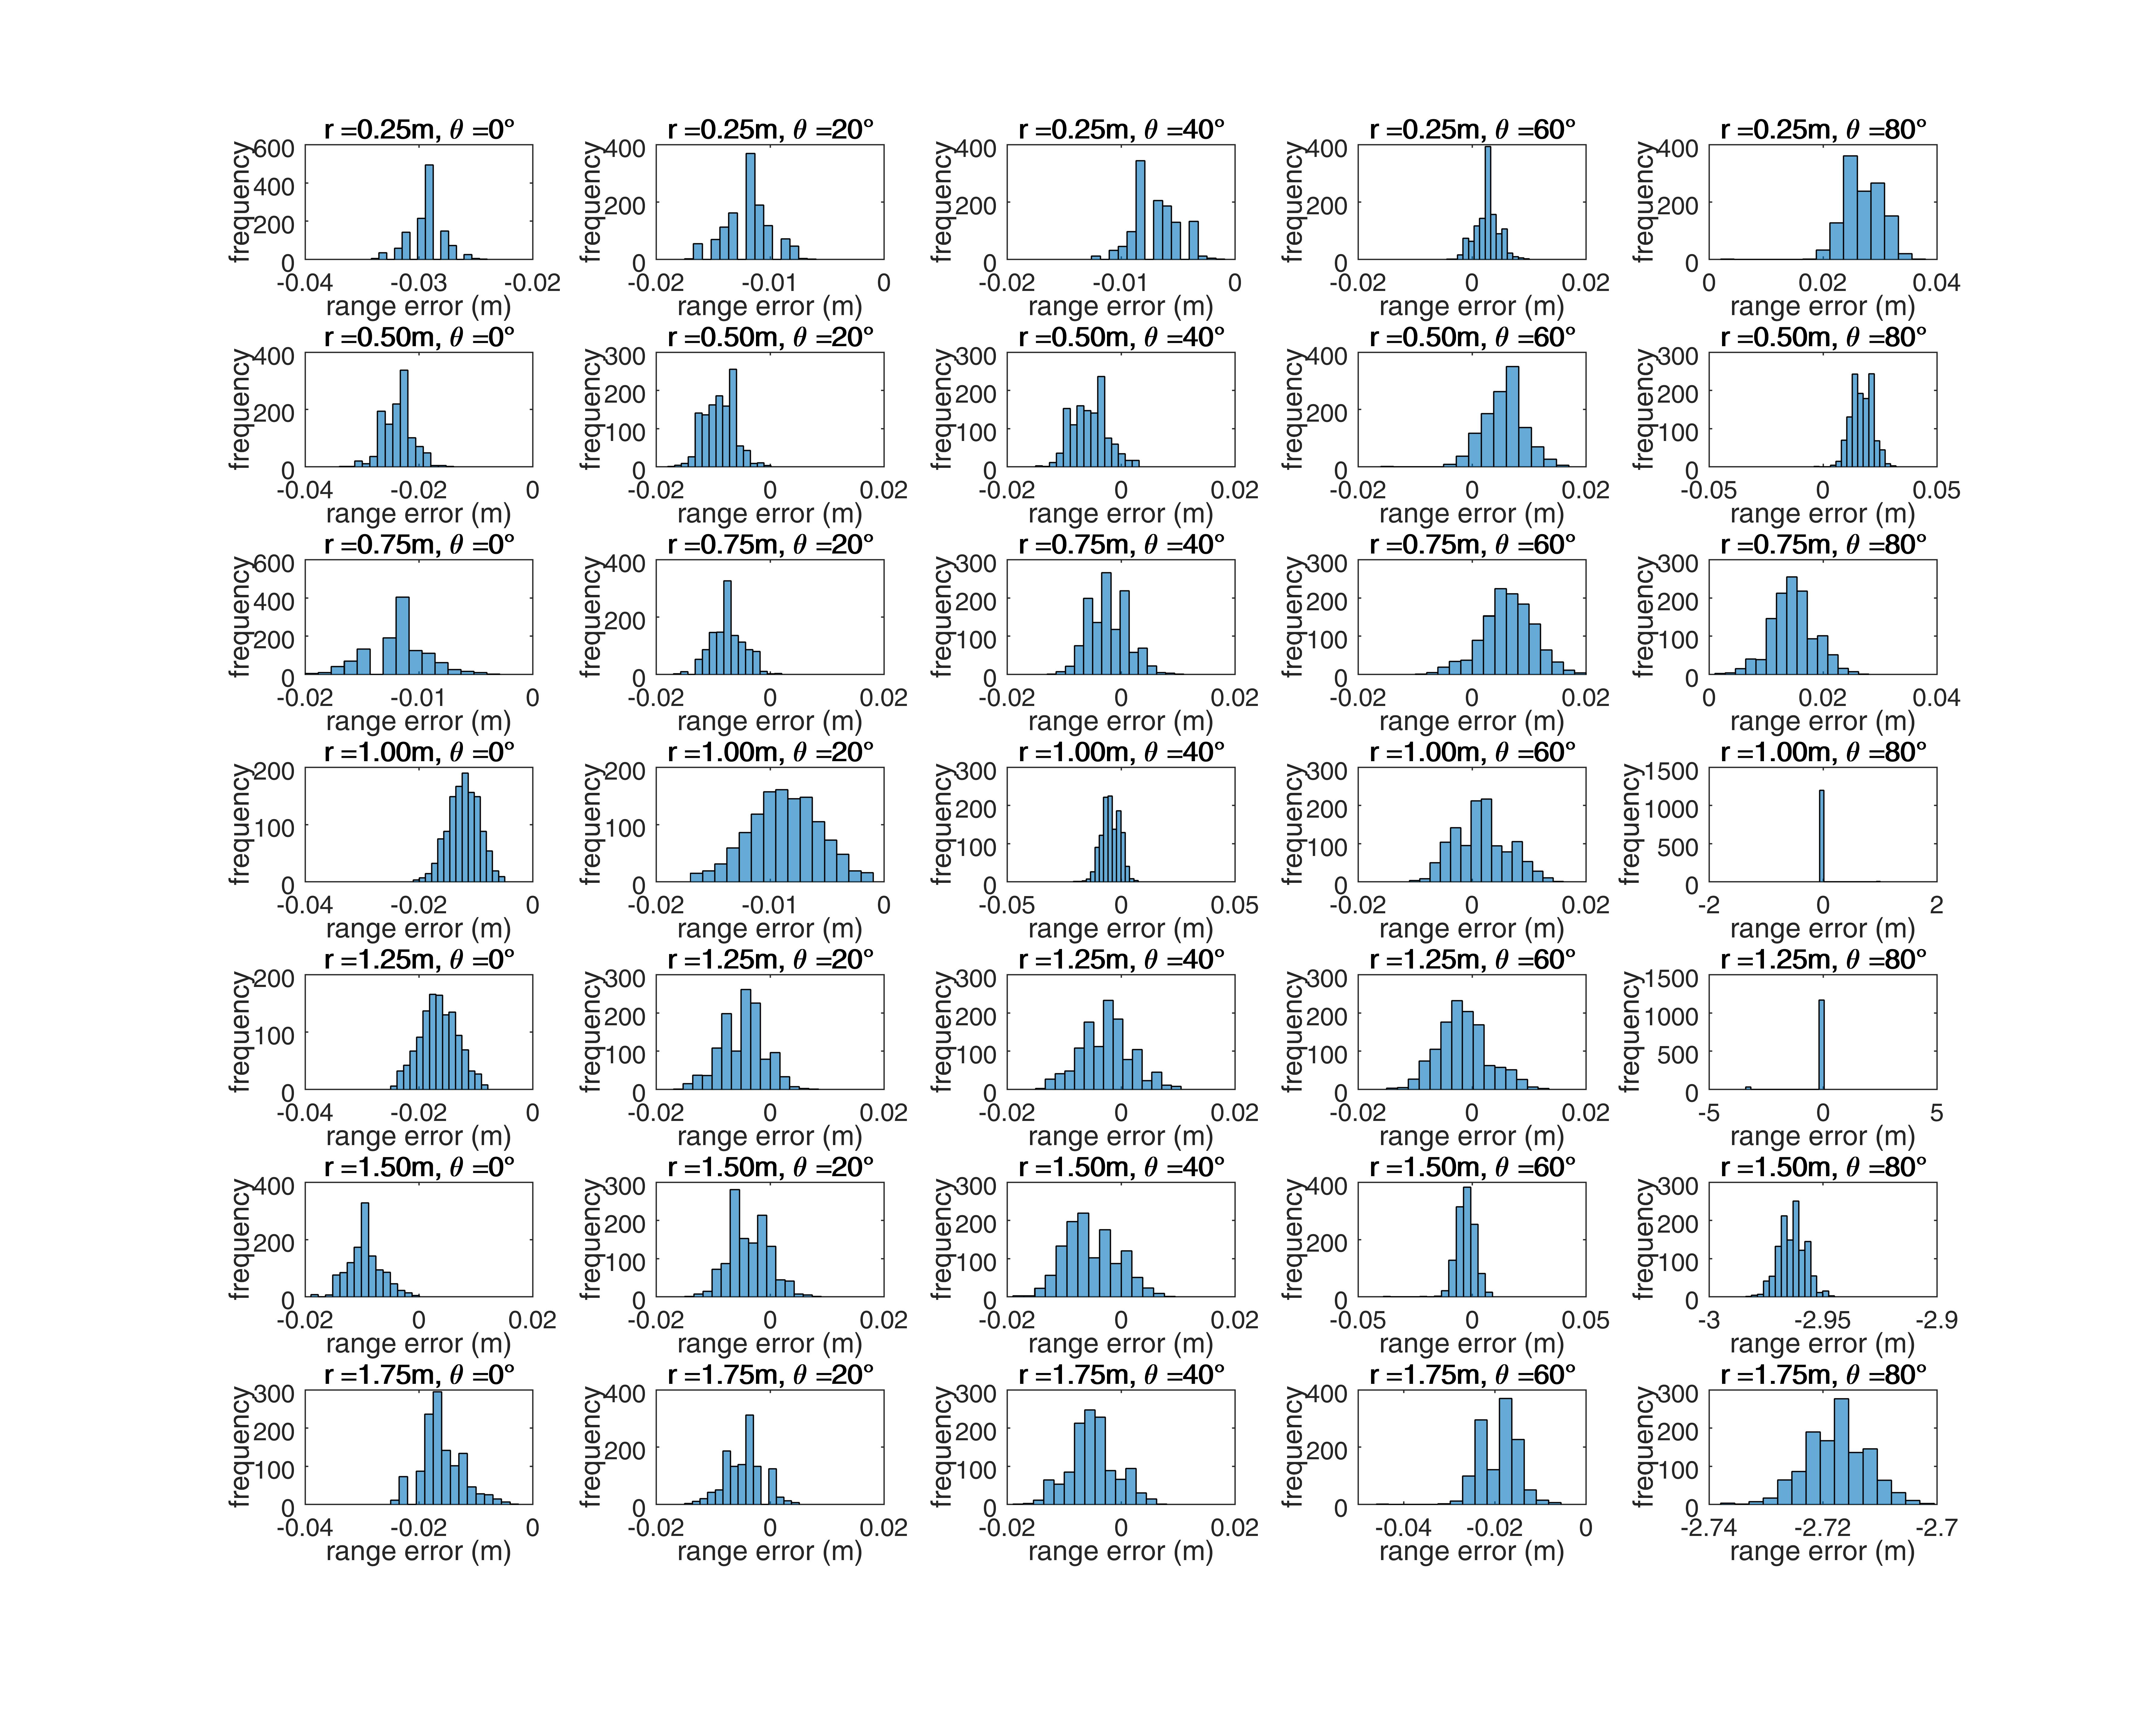
\includegraphics[width=1.25\textwidth,trim = 0mm 0mm 0mm 0mm,clip]{./Figures/range_error_histograms.jpg}
		  \caption{$r_{error}(r,\theta)$ approximately normally distributed}
		\end{figure}
		
		SHOW POINT CLOUD/SURFACE - range error mean vs $(r,\theta)$\\
		SHOW POINT CLOUD/SURFACE - range error standard deviation vs $(r,\theta)$\\		
		noise model
		
		*random walk surface noise model here too?\\
		surface properties (or sensor processing) error on mean range across surface, looks sinusoidal, peaks = 5mm deep \& 50mm wide approximately - seems to be independent of range and angle\\
		random walk model

\section{Testing Data Collection}
	\subsection{Setup}
		physical setup\\
		configurations/motions\\
		arm forward kinematics $\rightarrow$ cube pose\\
		estimate sensor angle with horizontal with wall calibration data		
		
	\subsection{Results}
		observer performance

